\documentclass[12pt,a4paper]{article}
\usepackage[margin=0.5in]{geometry}
\usepackage{graphicx}
\usepackage{floatrow}
\usepackage{authblk} 
\usepackage{etoolbox}
\usepackage{lmodern}

\date{}
\pagestyle{empty}

\makeatletter
\patchcmd{\@maketitle}{\LARGE \@title}{\fontsize{12}{19.2}\bfseries\@title}{}{}
\makeatother
\renewcommand\Authfont{\fontsize{12}{14.4}\selectfont}
\renewcommand\Affilfont{\fontsize{10}{10.8}\selectfont}

\title{\vspace{-15mm}\scalebox{0.9}[1.0]{Sampling in a hierarchical model of images reproduces top-down effects in visual perception}}
\author{\vspace{-2mm}Mih\'aly B\'anyai, Gerg\H{o} Orb\'an}
\affil{\vspace{-3mm}Computational Systems Neuroscience Lab, Wigner Research Centre for Physics, Budapest, Hungary}


\begin{document}

\maketitle
\thispagestyle{empty}

\vspace{-5mm}

Sensory perception can be understood as inference of latent causes underlying stimuli. This requires animals to learn the statistics of the environment in terms of a generative model with hierarchically organized latent variables corresponding to features of increasing complexity, which is characteristic of efficient probabilistic models (Hinton, 2006). While layers of probabilistic image models map intuitively to the hierarchical structure of the ventral stream, details of the correspondence have remained elusive.

Mean activity at the lowest level of visual hierarchy, V1 simple cells, are well covered by independent linear filters adapted to the statistics of natural scenes (Olshausen, 1996) further elaborated by introducing specific  dependencies between filters (Schwartz, 2001). Effects of top-down interactions on mean responses have been formalised in terms of covariance components of latent variables (Karklin, 2008). However, understanding the full response statistics of V1 neurons requires establishing computational principles that link efficient computations with higher-order statistics.

A computationally appealing and neurally feasible method to perform Bayesian inference is the construction of stochastic samples (Lee, 2003). Sampling establishes a link between the neural response distribution and probability distributions in Bayesian models. We explore sampling in a hierarchical model of vision and its consequences on neural response statistics.  

A hierarchical model of the visual system was built that bears similarities with Karklin's covariance model, and used sampling to perform Bayesian inference. Activity of model neurons were regarded as samples from the posterior distribution resulting from inference. Top-down effects in the visual hierarchy are particularly noticeable in the phenomenon of illusory contours, thus we used synthetic images with the model to predict the neural response to such stimuli. The sampling scenario predicts variance and covariance changes in V1 and reproduces magnitude modulation and temporal evolution of neural responses to real and illusory contours in V1 and V2. 

\vspace{5mm}

{\bf Three-layer model of the visual cortical hierarchy.} A key insight into the computational challenges faced by the visual system is coming from the observation of the uncertainty plaguing inference. The source of this uncertainty is partly attributed to noise that arises from variability in the environment or noise coming from our sensors. The other source of uncertainty is coming from ambiguity that is more and more prevalent as we go deeper in the hierarchy of inference. Coping with this ambiguity is key to efficient inference and an optimal treatment requires probabilistic computations. 
A successful line of research aims to identify image models efficient in performing tasks relevant to the visual system and then establish a link between activity between variables of the model and visual cortical cortical neurons. 
At the level of V1 Gaussian Scale Mixtures (GSM), that considers ambiguity in the contrast of natural images, could account for a wealth of data recorded from V1, including contrast invariance, non-classical receptive field effects (Schwartz, 2001) and response variance and covariance (Orb\'an et al, CoSyNe 2012). While at the level of V1 this form ambiguity can indeed be dominant, curbing other forms of ambiguities is essential for perception. Bayesian inference uses a prior distribution to tame ambiguities, which is learned from image statistics. In the case of the GSM the prior is the second-order statistics of linear filter activations, which indeed constrains  the sort of statistics and the forms of ambiguities it can account for. In order to retain the power of GSM but to enrich the form of prior over V1 activation and co-activation patterns we extended the GSM model by assuming a mixture of covariances to define context-specific dependencies of V1 neurons. Independent covariance components introduced an additional level of latent variables and inference was performed on this three-layer network (Fig. 1A).

Higher-level units ($g$) serve as coefficients for additive mixing of the $K$ components of the Gaussian covariance of the lower-level units ($v$): $P(v | g) = \mathcal{N}(v;0,C_v)$, where $C_v = \sum_{j=1}^K g_jC_j$. In turn, $v$-units define the Gaussian mean of pixels ($x$) through a set of linear filters ($A$), similar to Karklin \& Lewicki, 2008. The pixel statistics also depend on a scalar contrast variable ($z$) and an independent observation noise. $P(x|v,z) = \mathcal{N}(zAv,\sigma_x I)$. Prior densities of $g$ and $z$ are defined as fixed-parameter Gamma distributions, allowing us to produce synthetic data by defining all model parameters and conducting ancestral sampling. Importantly, Bayesian inference in this model yields a posterior probability distribution which explicitly formulates  uncertainties arising during inference. Representation of this posterior is assumed to achieved by a sequence of stochastic samples and  membrane potential of visual cortical neurons is assumed to map in these samples (Lee \& Mumford, 2003, Fiser et al, 2011). MCMC samples are obtained using a Gibbs sampling scheme. 

%\begin{eqnarray}
%p(v \mid x,g,z) = \mathcal{N}\left(v; \frac{z}{ \sigma_x} \left( \frac{z^2}{ \sigma_x} A^T A + C_v^{-1}\right)^{-1} A^T x, \left(\frac{z^2}{\sigma_x} A^T A + C_v^{-1}\right)^{-1}\right) \\
%\log p(g \mid X,V) \sim -\frac{1}{2} \left[\log(\det(C_v)) + v^T C_v^{-1} v \right] + (\alpha-1) + \log p(g) \\
%\log p(z \mid X,V) \sim -\frac{1}{2} \left[ D_x\log(\sigma_x) + \frac{1}{\sigma_x}  (x - zAv)^T (x - zAv)\right] + \log p(z)
%\end{eqnarray}
%
%The conditional posteriors of g and z need to be sampled by MCMC steps themselves. 
Priors over V1 activations are imposed by the activation of latent variables $g$, that need to be adapted to the environment. We trained our network on natural images to learn the elements of the covariance component matrices from data in an unsupervised manner by  a generalised expectation-maximisation scheme. 
%This provides a candidate procedure to model the data-driven acquisition of covariance components characteristic to natural stimuli, which we validated on synthetic datasets. 
The fact that the model can learn multiple correlational contexts and infer their composition contributing to an image patch not only extends the power of this image model but also extends the spectrum of phenomena in neural response statistics relative to single-covariance models such as Gaussian Scale Mixtures (Schwartz \& Simoncelli, 2001).  Since the model captures higher-order statistics  through the mixture of covariance components, it becomes possible to learn and perceive multiple spatially overlapping covariance structures instead of learning an average over the complete image statistics. Importantly, the form of ambiguities that the proposed image model can capture can be  understood as formalisations of Gestalt effects observed in psychology under a wide range of circumstances that are characterised by impoverished information. 

{\bf Prediction of responses to illusory contours.} The model makes predictions on context-dependent changes in mean responses and also the variance and correlation structure of the response distribution. Top-down effects can also be captured in the timing of responses. A prominent form of top-down effect is the perception of illusory contours (IC). Neurons in V1 are sensitive to illusory contours and the timing of such responses is delayed compared to responses to edge-defined contours, and the appearance of IC-evoked responses in the secondary visual cortex (V2) precedes that in V1  (Lee \& Nguyen, 2001). Synthetic stimuli consisting of line segments with an  occluded receptive field of a selected V1 neuron  was constructed  (Fig. 1B) and  Gibbs sampling yielded a time series for cell activations (Fig. 1C). As the activation of a $g$ variable, which corresponds an extended line segment,  activated the $v$-unit in a top-down manner,  trajectories reproduced the measured magnitude ratio and timing of IC responses. Such selective activation of correlated units requires the learning of statistics of higher than second order, which is achieved by the multiple components, extending the predictive power of models learning a single covariance matrix, such as GSM. Predictions on context-dependent changes in trial-to-trial variability and noise correlation of V1 neurons are wide and some waiting experimental confirmation but can account for perceptual phenomena documented in
 Gestalt literature. 

\begin{figure}[h]
\floatbox[{\capbeside\thisfloatsetup{capbesideposition={right,top},capbesidewidth=6cm}}]{figure}[\FBwidth]
{\caption{{\bf A.} Outline of the covariance component model. {\bf B.} Two overlapping components of the test model (top),  stimulus and the percept of the model formed by posterior samples (bottom). {\bf C.} Time evolution of samples from $v$-units with receptive fields at stimulated, occluded and other stimulus part and the $g$-unit with the left covariance component. Red line indicates beginning and end of stimulus presentation. Approximate timescale based on typical correlation length in V1. {\bf D.} Reproduction of V1 responses to IC and line stimuli from Lee \& Nguyen, 2001.
}\label{fig:test}}
{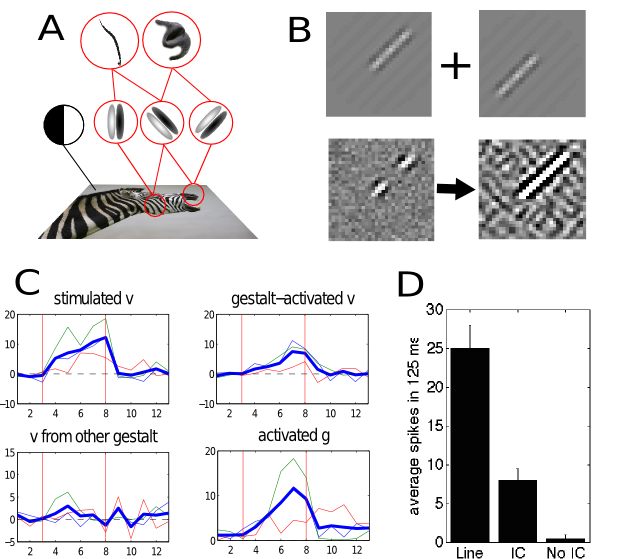
\includegraphics[width=10cm]{cosyne_figure.png}}
\end{figure}


\end{document}
